\documentclass{article} % For LaTeX2e
\usepackage{nips14submit_e,times}
\usepackage{hyperref}
\usepackage{url}
\usepackage{amsmath}
\usepackage{amssymb}
\usepackage{bbm}
\usepackage{tikz}
\usepackage{tikz-qtree}
\usepackage[sort&compress]{natbib}
\usepackage{natbibspacing}
\usepackage{multirow}
\usepackage{subcaption}

\usetikzlibrary{arrows}
\usetikzlibrary{shapes, trees}

\bibliographystyle{unsrt}

\DeclareMathOperator*{\argmax}{argmax}
\DeclareMathOperator*{\argmin}{argmin}

\newcommand{\unorderedS}{\mathcal{S}^{\mathrm{u}}}
\newcommand{\orderedS}{\mathcal{S}^{\mathrm{o}}}
\newcommand{\ourmethod}{NCL}

\newcommand{\bmcomment}[1]{\textcolor{blue}{\textsc{\textbf{[#1 --bm]}}}}
\newcommand{\nascomment}[1]{\textcolor{red}{\textsc{\textbf{[#1 --nas]}}}}
%\documentstyle[nips14submit_09,times,art10]{article} % For LaTeX 2.09


\title{Learning Not to Try Too Hard}

\author{
Bill McDowell\thanks{Alternative email: \texttt{forkunited@gmail.com}} \\
School of Computer Science\\
Carnegie Mellon University\\
Pittsburgh, PA 15213 \\
\texttt{wmcdowel@cs.cmu.edu} \\
\And
Noah A.~Smith \\
School of Computer Science\\
Carnegie Mellon University\\
Pittsburgh, PA 15213 \\
\texttt{nasmith@cs.cmu.edu} \\
}

% The \author macro works with any number of authors. There are two commands
% used to separate the names and addresses of multiple authors: \And and \AND.
%
% Using \And between authors leaves it to \LaTeX{} to determine where to break
% the lines. Using \AND forces a linebreak at that point. So, if \LaTeX{}
% puts 3 of 4 authors names on the first line, and the last on the second
% line, try using \AND instead of \And before the third author name.

\newcommand{\fix}{\marginpar{FIX}}
\newcommand{\new}{\marginpar{NEW}}

\nipsfinalcopy % Uncomment for camera-ready version

\begin{document}

\maketitle

%\bmcomment{It seems like a lot of other papers refer to 'cost' as 'loss'... 
%Is there somewhere where people call it 'cost' like we are?}
%\nascomment{will address this}

%\begin{abstract}
%\nascomment{do last}
%\end{abstract}

\section{Introduction}

Discriminative learning algorithms are often motivated by their
ability to trade off among different kinds of prediction mistakes with
different costs.  The cost of a mistake is usually taken to be fully
defined by the task, i.e., human system designers are trusted to
encode this knowledge prior to learning.  Information about the
inherent ease of avoiding some errors vs.~others is generally not
taken into account.   Closely related to this, and critically
important in domains where the data is constructed by humans, is the
problem that the outputs in the training data may be unreliable.  For
example, if training data is produced by asking humans to label
instances, and two labels are insufficiently well defined for human
labelers to distinguish them,
then a learner might be forgiven for conflating them.

We consider situations where human intuition about relative costs of
different errors is insufficient.  In a margin-based linear modeling
framework, we propose a method for incorporating \textbf{learning of
  the cost function} alongside learning of the model.  Our approach
introduces explicit estimates of the ``ease'' of avoiding each type of
error
(for a particular model family).   For error types that are ``just too
hard,'' our model is offered the possibility of giving up in favor of
making other, less challenging predictions more accurately.

In practice, we found that our current method performs with 
approximately the same accuracy as a baseline SVM on text 
classification tasks, but it is able learn cost functions
that intuitively make sense.

%\bmcomment{Might want to give some motivating examples? Not sure if that's
%necessary or not. One example of multiclass domain, and one example where
% cost functions are used in structured domains} 

% \bmcomment{Mention examples of measures of 'difficulty'? Cite.}

%

\section{Background and Notation}

In a prediction problem, let $\mathcal{X}$ denote the input space,
$\mathcal{Y}$ denote the output space, and assume $N$ training
instances $\{(x_1, y_1), \ldots, (x_N, y_N)\}$.  We assume a linear
model and prediction function:
\begin{equation}
\hat{y} = \argmax_{y \in \mathcal{Y}} \left(f(x, y;\mathbf{w}) \triangleq \mathbf{w}^\top \mathbf{g}(x, y) \right)
\end{equation}
where $\mathbf{w} \in \mathbb{R}^D$ are the parameters to be learned
and $\mathbf{g} : \mathcal{X} \times \mathcal{Y} \rightarrow
\mathbb{R}^D$ is the feature vector function.  We will let
$\mathcal{M} =\{f(\cdot,\cdot;\mathbf{w}) \mid \mathbf{w} \in
\mathbb{R}^D\}$ denote the model family under consideration, given a
fixed choice of $\mathbf{g}$.

Our approach, which assumes $\mathcal{Y}$ is categorical, is based on
the soft margin formulation of multiclass support vector machines
\citep{vapnik1998statistical,crammer2002algorithmic,weston1998multi}.
Tsochantaridis et al.~\citep{tsochantaridis2004support} and Taskar et
al.~\citep{koller2003max} generalized this framework to allow for
differences in costs between different kinds of mistakes, as found
when $\mathcal{Y}$ is structured.  Let the cost function
$\Delta:\mathcal{Y}\times\mathcal{Y}\rightarrow\mathbb{R}$  be such
that $\Delta(y, y')$ is the cost of predicting $y$ when the correct
label is $y'$.  We use the ``margin rescaling'' variant of the multiclass SVM:
\begin{align}
 \min_{\boldsymbol{\xi}\geq 0, \mathbf{w}}
\frac{\lambda}{2}\|\mathbf{w}\|_2^2+\frac{1}{m}\sum_{i=1}^N\xi_i 
 \text{\ \ \ s.t.\ \ \ } \forall i,  \forall y \in \mathcal{Y} \setminus
 \{y_i\},  f(x_i, y_i; \mathbf{w}) - f(x, y, \mathbf{w}) \geq
 \Delta(y, y_i) - \xi_i \label{marginRescaling}
\end{align}
This objective seeks $\mathbf{w}$ that minimizes misclassifications while
maximizing the margin between correct and incorrect instances.
Further, the more incorrect an $(x,y)$ pair is, the greater the margin
should be.  This problem is often transformed into an unconstrained
one corresponding to direct minimization of the regularized average
hinge loss:
\begin{equation}
\label{svmObjective}
\min_{\mathbf{w}} \frac{\lambda}{2}\|\mathbf{w}\|_2^2 +
\sum_{i=1}^N  -f(x_i, y_i; \mathbf{w}) + \max_{y \in \mathcal{Y}}
  f(x_i, y; \mathbf{w}) + \Delta(y, y_i)
\end{equation}

We introduce some notation for errors.
We let $\mathcal{S} \subseteq 2^{\mathcal{Y}\times\mathcal{Y}}$ be a
collection of prediction error classes that 
exhausts $\mathcal{Y}^2$ (i.e., $\bigcup_{S \in
  \mathcal{S}} S = \mathcal{Y}^2$); the error 
  classes need not be
mutually exclusive.  We let $e_{S} \in \mathbb{R}$ denote an estimate
of the ``ease'' with which a learner searching in $\mathcal{M}$ 
can successfully avoid errors in class $S$.  Then we let:
\begin{equation}
\Delta(y, y') = \sum_{S \in \mathcal{S}: (y, y') \in S} e_S =
\mathbf{e}^\top \mathbf{s}(y, y')
\end{equation}
where $\mathbf{e}$ is a vector of the $e_S$ and $\mathbf{s}$ is a
binary vector of length $\mathcal{S}$ indicating which error class(es)
each possible confusion in $\mathcal{Y}\times\mathcal{Y}$ belongs to.

In this paper, we consider two prediction error classes, corresponding
to unordered and ordered pairs of outputs.  We denote them
$\unorderedS$ and $\orderedS$, respectively.  

% There are many possible choices for prediction classes $\mathcal{S}$, but
% in this paper, we focus on the following two:

% \begin{equation}
% \begin{split}
% & \mathcal{S}_{[\mathcal{Y}]^2} = \{ S_{\{\mathbf{y},\mathbf{y}'\}} | \mathbf{y},\mathbf{y}'\in\mathcal{Y}\} \\
% \text{ where } & S_{\{\mathbf{y},\mathbf{y}'\}}=
% \{ (\mathbf{y}_1, \mathbf{y}_2) | (\mathbf{y}_1=\mathbf{y}\wedge \mathbf{y}_2=\mathbf{y}')\vee(\mathbf{y}_1=\mathbf{y}'\wedge \mathbf{y}_2=\mathbf{y}) \} \\
% \end{split}
% \end{equation}

% \begin{equation}
% \mathcal{S}_{\mathcal{Y}^2} = \{ S_{(\mathbf{y},\mathbf{y}')} | \mathbf{y},\mathbf{y}'\in\mathcal{Y}\}\text{ where }S_{(\mathbf{y},\mathbf{y}')}=\{ (\mathbf{y},\mathbf{y}') \} \\
% \end{equation}

% $\mathcal{S}_{[\mathcal{Y}]^2}$ contains a prediction class for every
% unordered pair of labels, and $\mathcal{S}_{\mathcal{Y}^2}$ contains
% a prediction class for every ordered pair.  We might choose 
% $\mathcal{S}_{[\mathcal{Y}]^2}$ when factoring the cost function if
% we believe it is equally easy to resolve misclassifications of 
% $\mathbf{y}$ as $\mathbf{y}'$ and misclassifications of $\mathbf{y}'$
% as $\mathbf{y}$.  Otherwise, if we suspect these two incorrect 
% prediction types to differ in easiness, then we might choose 
% $\mathcal{S}_{\mathcal{Y}^2}$.

\section{Cost Learning Model}
\label{costLearningModel}


Previous work assumes $\Delta$ follows intuitively from the prediction
task.  For example, in natural language dependency parsing, the number
of words attached to the wrong parent (Hamming distance for the parse
tree) is a sensible choice.  
We propose to parameterize $\Delta$ and
learn its parameters jointly with $\mathbf{w}$.  This learned cost
function should encode distances between outputs from the perspective
of the ease with which a model in the family $\mathcal{M}$
can distinguish between them.
This joint learning setup is expected to be particularly useful when
some classes of errors are difficult or impossible for a model in the
class to resolve, due to unreliable annotations or an insufficient
choice of features $\mathbf{g}$.


\subsection{Ease}
\label{sec:ease}
We desire a model that estimates prediction ease $\mathbf{e}$ while
estimating
predictive model parameters $\mathbf{w}$. 
We have used the term ``ease''
with respect to an arbitrary model in the family $\mathcal{M}$, but it
is more sensible to consider the particular model we seek to
estimate.  We propose that, for error class $S$ and a model with
parameters $\mathbf{w}$, ease $e_S$ should be inversely related to the
number of
of margin violations involving $S$ that $f(\cdot, \cdot; \mathbf{w})$ makes in the
training data assuming that $\argmax$ always gives a 
single label, breaking ties arbitrarily:

\begin{equation}
v_S (\mathbf{w}, \mathbf{e}) \triangleq \left|\left\{ i  \in \{1,\ldots, D\} \mid \left(y_i, \textstyle \argmax_{y \in \mathcal{Y}} f(x_i, y ; \mathbf{w}) +
\mathbf{e}^\top \mathbf{s}(y, y_i)\right) \in S\right\}\right| \label{eq:set}
\end{equation}

The intuition is that, when $v_S(\mathbf{w},\mathbf{e})$ 
is large, it is because it is not easy for the
model to shrink.  Of course, we should also take into account 
that the distribution of the data may make some errors more frequent,
inflating the size of the set in Eq.~\ref{eq:set} even if $S$ is ``easy.''
Further,  \emph{infrequently} observed labels are generally
expected to be harder to predict.  Yet for an $S$ that includes errors on
a  rarely occurring class, the set in Eq.~\ref{eq:set} will
necessarily be small, regardless of how easy it is.
We therefore propose the following condition for $e_S$:
\begin{equation}
e_S = \max\left( 0, 1 - \frac{v_S(\mathbf{w}, \mathbf{e}) }{n_S}\right) \label{e-condition}
\end{equation}
where $n_S$ is a fixed, \emph{a priori} upper bound on the count of
$S$ errors, $v_S$.   This
has the desirable property that  if $v_S \ge n_S$,  i.e., $S$ is too
difficult to shrink, then ease $e_S$ goes to zero and the model is
allowed to give up on $S$.  It also keeps $e_S \in [0,1]$, 
ensuring interpretability of the ease relative to the
maximum possible value of $e_S=1$.

% The size of $S_{\mathcal{M},\mathbf{g},D}$ is the number of
% training examples with margin violations in class $S$. If
% the size of this set is large, we might infer that the
% model has trouble shrinking it, and so it's not 'easy'.  This 
% might lead us to conclude that $S_{\mathcal{M},\mathbf{g},D}$ 
% tends to shrink with 'easiness'.  However,
% for many data sets and choices of $\mathcal{S}$, the size 
% of each $S_{\mathcal{M},\mathbf{g},D}$ can be inherently
% biased by the data independently of 'easiness'.  For example, 
% for $S_{\{\mathbf{y},\mathbf{y}'\}}\in\mathcal{S}_{[\mathcal{Y}]^2}$, 
% the size of $S_{\{\mathbf{y},\mathbf{y}'\},\mathcal{M},\mathbf{g},D}$ 
% is biased by the number of examples in the training data which have 
% output labels $\mathbf{y}$ and $\mathbf{y}'$--if there are few 
% training examples of labels 
% $\mathbf{y},\mathbf{y}'\in\mathcal{Y}$, then the size of 
% $S_{\{\mathbf{y}, \mathbf{y}'\},\mathcal{M},\mathbf{g},D}$ 
% will necessarily be small relative to other prediction classes.
% Furthermore, we expect 
% output labels which occur infrequently in the training data to 
% be more difficult for the model to predict correctly, so this
% will lead to the size of 
% $S_{\{\mathbf{y},\mathbf{y}'\},\mathcal{M},\mathbf{g},D}$ 
% increasing with the 'easiness' of 
% $S_{\{\mathbf{y},\mathbf{y}'\}}$ which is opposite the 
% conclusion that that we draw if we think of the size of 
% $S_{\{\mathbf{y},\mathbf{y}'\},\mathcal{M},\mathbf{g},D}$ as
% increasing due to the model's difficulty in shrinking it.  In general, 
% this suggests that if we want the size of $S_{\mathcal{M},\mathbf{g},D}$
% to vary with easiness, we need to normalize it to account for 
% properties of the training data that introduce irrelevant
% biases.  

\subsection{Objective}

Our approach is a modification to the SVM objective in
Eq.~\ref{svmObjective}; it is a joint optimization of $\mathbf{w}$ and $\mathbf{e}$:
\begin{equation}
\label{costObjective}
\min_{\mathbf{e}\geq 0,\mathbf{w}} \frac{\lambda}{2}\|\mathbf{w}\|_2^2
+ \frac{1}{2} \|\mathbf{e}\|_{\mathbf{n}}^2 - \mathbf{e}^\top
\mathbf{n} + \sum_{i=1}^N -f(x_i,y_i; \mathbf{w})  + \max_{y \in
  \mathcal{Y}} f(x_i,y ; \mathbf{w}) + \mathbf{e}^\top \mathbf{s}(y, y_i)
\end{equation}
where $\mathbf{n}$ is the vector of upper bounds on prediction error
frequencies and 
$\|\mathbf{e}\|_{\mathbf{n}}^2 = \sum_{S \in
  \mathcal{S}} n_Se_S^2$.\footnote{$\|\cdot\|_{\mathbf{n}}$ norm is
  a Mahalanobis norm, as described in
  \citep{mahalanobis1936generalized}.} 
 The modification amounts to (1) including
$\mathbf{e}$ as a free variable and (2) regularizing it with a quadratic
penalty (second term in Eq.~\ref{costObjective}) and a linear ``reward''
(third term in Eq.~\ref{costObjective}).  The linear penalty selects
which $e_S$ should be nonzero---equivalently, are not impossibly
difficult. Setting $e_S=0$ amounts to giving up on $S$
errors.\footnote{The meaning of ``giving up'' is unclear.  It seems
that setting $e_S=0$ actually amounts to giving up on margin maximization,
but not error minimization with respect to $S$, but we don't work 
this out in detail.\bmcomment{Noah, do you understand
this differently?}}

Most importantly, Eq.~\ref{costObjective} is minimized at ease
 $\mathbf{e}$ 
that matches Eq.~\ref{e-condition}.  To see this, we define 
$C(\mathbf{w},\mathbf{e})$ as the objective minimized in 
Eq~\ref{costObjective}, and derive the optimal ease 
values $\mathbf{e}^*$
such that $\mathbf{0}\in \partial C(\mathbf{w}^*,\mathbf{e}^*)$.  
The subdifferential $\partial C$ is given by:\footnote{See
 \url{http://see.stanford.edu/materials/lsocoee364b/01-subgradients_notes.pdf} for help in understanding subgradients.}

\begin{equation}
\label{subdifferential}
\begin{split}
\partial C(\mathbf{w},\mathbf{e}) = & \frac{\lambda}{2}\nabla (\|\mathbf{w}\|_2^2)
+\frac{1}{2}\nabla (\|\mathbf{e}\|^2_{\mathbf{n}})-\nabla (\mathbf{e}^\top \mathbf{n})
+ \\ 
& \sum_{i=1}^N -\nabla (f(x_i,y_i; \mathbf{w}))+ 
\mathbf{Co}(\nabla F^{\Delta}_{\max}(x_i,y_i;\mathbf{w},\mathbf{e}))
\end{split}
\end{equation}

Where addition and subtraction operators are overloaded to perform 
additions and subtractions over sets, 
$\mathbf{Co}(\cdot)$ gives the convex hull, and 
$\nabla F^{\Delta}_{\max}$ is defined as:

\begin{equation}
\label{FmaxDef}
\nabla F^{\Delta}_{\max}(x,y;\mathbf{w},\mathbf{e}) = 
\{ \nabla f(x, \hat{y} ; \mathbf{w}) +
\nabla \mathbf{e}^\top \mathbf{s}(y, \hat{y})
| \hat{y}\in\argmax_{y' \in \mathcal{Y}} f(x, y' ; \mathbf{w}) +
\mathbf{e}^\top \mathbf{s}(y, y') \}
\end{equation}

We are only interested in the value of $\mathbf{e}$, so
we can consider Eq.~\ref{subdifferential} reduced to 
a simpler subdifferential 
with respect to a single component $e_S$ of $\mathbf{e}$:

\begin{equation}
\label{eSubdifferential}
\partial_{e_S} C(\mathbf{w},\mathbf{e}) = 
n_S e_S -n_S+
\sum_{i=1}^N 
\mathbf{Co}(\frac{\partial 
F^{\Delta}_{\max}(x_i,y_i;\mathbf{w},\mathbf{e})}{\partial e_S})
\end{equation}

Given that $\mathbf{0}\in \partial C(\mathbf{w}^*,\mathbf{e}^*)$,
Eq~\ref{eSubdifferential} leads to:

\begin{equation}
\label{optimal-e}
e_S^*\in 1 - \frac{\sum_{i=1}^N 
\mathbf{Co}(\frac{\partial 
F^{\Delta}_{\max}(x_i,y_i;\mathbf{w}^*,\mathbf{e}^*)}{\partial e_S})}{n_S}
\end{equation}

If we allow the $\argmax$ in Eq.~\ref{FmaxDef} to arbitrarily break
ties as in Section~\ref{sec:ease}, and we constrain $e^*_S\geq 0$ as in
Eq.~\ref{costObjective}, then Eq.~\ref{optimal-e} suggests that 
$e^*_S$ takes on the value given by Eq.~\ref{e-condition} when the
objective is minimized.  So our objective chooses values of 
$\mathbf{e}$ according to our intuitions from Section~\ref{sec:ease}.

%At points of the objective in Eq.~\ref{costObjective} that are 
%differentiable with respect to $e_S$, then it is
%traightforward to show that Eq.~\ref{e-condition} holds.  At
%non-differentiable points, which occur due to ties among $y$, $e_S$ will lie
%between the values given by Eq.~\ref{e-condition} for these tied $y$.

%\bmcomment{Is this non-differentiable part understandable?  Is it enough,
%or do I need to give the proof?  I still haven't actually gone through
%the proof completely, so maybe we should at least go over the reasoning
%to make sure I'm not crazy.} \nascomment{I think we should add the
%proof.  the paper is short, so there is room, at least right now.
%might be okay just to give the proof for differentiable case.}


\subsection{Constants \textbf{n}}

The appropriate choice for the normalization vector $\mathbf{n}$ in 
Eq.~\ref{costObjective} depends on the prediction classes in
$\mathcal{S}$ and the types of bias we seek to avoid when estimating $\mathbf{e}$.
For $\unorderedS$ and $\orderedS$, we are most concerned with
unbalanced marginal distributions over labels.  
Let $c_y$ be the frequency of the label $y$ in the training data,
$|\{i \mid y_i = y\}|$.
We propose two choices
of $\mathbf{n}$, both based on the training data:
\begin{enumerate}
\item \textbf{Logical} $\mathbf{n}$:  an upper bound on $v_S(\cdot,
  \cdot)$ based on frequencies in the training data.  For $\unorderedS$, let
  $n_{S_{\{y,y'\}}} = c_y+c_{y'}$.  For
  $\orderedS$, let $n_{S_{y, y'}} = c_y$ where
  $S_{y,y'}$ corresponds to an erroneous label of $y'$ in place of the
  correct $y$.
\item \textbf{Expected} $\mathbf{n}$:  an upper bound calculated by
  assuming that our learner can perform better than a random
  classifier that uses label proportions observed in the training
  data.    For $\unorderedS$, let $n_{S_{\{y,y'\}}} = 2c_y c_{y'} / N$.  For
  $\orderedS$, let $n_{S_{y,y'}} =  c_y c_{y'} / N$. 
\end{enumerate}

 The \textbf{Logical} choice
will tend to dramatically overestimate the maximum count of each
prediction error,
but we might choose it over \textbf{Expected} if we
believe that the random classifier would not give a baseline rate at
which our model is biased to predict certain labels by the label
distribution independent of the inputs.
A third option, not explored here, might use a more sophisticated
model to estimate bounds on error counts.

\section{Experiments}

We implemented the multiclass SVM (Eq.~\ref{svmObjective}) and
variations of our method---which we refer to as
normalized cost learning (\ourmethod{}; Eq.~\ref{costObjective})---
and we compared each of these implementations on standard text
classification datasets in several experiments.  In each experiment, 
we used a standard train/test split for the dataset, but with 10\% of
the training set held out to perform a grid search for $\lambda$ over
16 values in $[10^{-6}, 50]$, choosing the value that
gives the best accuracy, and then fixing $\lambda$ and
retraining on the whole training set.  For training,
ran 
stochastic gradient descent (SGD) with a learning rate determined
by AdaGrad for 50 passes over random permutations of the data
\citep{yin2003stochastic}\citep{duchi2011adaptive}.  We observed that 
during the last ten
passes, accuracy varied by $<
0.01$ and fewer than 10\% of predictions changed.\footnote{
We were running for 150 iterations for previous buggy
versions of the models, but we adjusted down to 50 iterations 
as our remaining working time began to dwindle, and we realized 
that these experiments were going to give negative results.  It's
 unlikely that increasing the number of iterations from 50 will
change the current conclusions, but if this work is ever published,
we might want to rerun the algorithms with more iterations---just 
to be safe.
}

\subsection{Datasets}

We considered two datasets with relatively large output label sets:
20 Newsgroups (20NG; 20 category labels corresponding to newsgroups)
\footnote{\url{http://qwone.com/~jason/20Newsgroups}} and Reuters-21578
(R52; 52 topic labels).
\footnote{\url{http://www.csmining.org/index.php/r52-and-r8-of-reuters-21578.html}.}    
We followed \citep{2007:phd-Ana-Cardoso-Cachopo} in
preprocessing the text corpora (including downcasing, removing
symbols, etc.), and we let features in $\mathbf{g}$ correspond to tf-idf 
computed over unigrams \citep{lan2006proposing}.
\footnote{We also ran experiments
on synthetic data sets, but the results for those experiments are similar
to the results for the text-classification data sets, and 
so they are not included in this document. Specifically, the synthetic data
set results show at most minor performance gains on some versions of the data
although the cost function seems to be learned appropriately.
Furthermore, the synthetic data includes only four features in each task,
which is unrealistic, and causes SGD difficulty in convergence
due to the model's predictions being super sensitive to 
each weight.\bmcomment{Does this make sense?}  In the 
future, it would be 
beneficial
to extend these datasets to include tasks with many more
features,
and use them to make sure our current cost learning models 
are 
functioning properly.
 See the code documentation
at \url{https://github.com/forkunited/CostFunctionLearning/} for more 
detail on how to use and generate the synthetic data.}

The 20NG dataset consists of 18,846 documents, sorted by date, with
60\% used for training.  Though the categories are roughly uniformly
distributed, the topics vary greatly in their relatedness, following a
hierarchical labeling scheme (e.g., \emph{rec.autos} and
\emph{rec.motorcycles} are likely more closely related than either to
\emph{sci.space}).  This offers a way to measure the effectiveness of
\ourmethod{} at learning ``ease'':   the less closely related two 
categories are, the greater the ease in learning to distinguish them.

The R52 dataset contains 9,100 documents; we use the ModApte split
(70\% training).  The label distribution is skewed, with 43\% of
documents assigned to \emph{earn} and 37 topics
receiving fewer than 50 examples.


\subsection{Results}

Table~\ref{accuraciesTable} shows the micro-averaged
accuracies on the Reuters and 20 newsgroups tasks for the 
SVM baseline model and \ourmethod{} with
various prediction error classes
($\unorderedS$; $\orderedS$) and normalization constants
($\boldsymbol{1}$, i.e., none; logical; expected).  
We had expected that \ourmethod{} might give an overall
increase in accuracy on each task, but unfortunately, \ourmethod{} 
generally gave approximately the same accuracy as  
the SVM, which
suggests that the learned cost-scaled
margins did not help \ourmethod{} to generalize better than 
the 
SVM's constant margin.  

\begin{table}[t]
\caption{Micro-averaged accuracies of different
  learners.}
\label{accuraciesTable}
\begin{center}
\begin{tabular}{l|rr|r}
\multirow{2}{*}{\bf Learner}          &  \multicolumn{2}{c|}{\bf 20NG} & \multirow{2}{*}{\bf{R52}} \\
                                      & \bf{full} & \bf{clusters}      & 
\\ \hline 
SVM                                   & 0.834     & 0.920              & 0.945 \\
\ourmethod{}: $\orderedS$, none       & 0.834     & 0.919              & 0.946 \\ 
\ourmethod{}: $\unorderedS$, none     & 0.832     & 0.921              & 0.945 \\
\ourmethod{}: $\orderedS$, logical    & 0.836     & 0.920              & 0.948 \\ 
\ourmethod{}: $\unorderedS$, logical  & 0.830     & 0.919              & 0.948 \\
\ourmethod{}: $\orderedS$, expected   & 0.830     & 0.920              & 0.949 \\ 
\ourmethod{}: $\unorderedS$, expected & 0.820     & 0.911              & 0.946 \\
\end{tabular}
\end{center}
\end{table}

We had especially hoped to see accuracy
gains in the ``clusters'' column under ``20NG''.  Whereas the 
``full'' column shows accuracies computed over all categories
 in the 20 newsgroups task, the ``clusters'' column
shows accuracies computed with all categories from a single
topical cluster mapped to a single label---where the topical
clusters are shown in Figure~\ref{clusters} and
defined at \url{http://qwone.com/~jason/20Newsgroups/}.  
Assuming
\ourmethod{}'s learned cost function gives 
higher costs for 
mislabelings between topical clusters and lower 
costs for mislabelings
within topical clusters, we had 
expected that the model would focus
on adjusting its feature weights 
to distinguish between categories
in separate clusters, which would have 
resulted in an overall increase in
 accuracy in the ``clusters'' column.  
 
We inspected the learned cost functions from 
the $\unorderedS$ versions of \ourmethod{} 
to check our assumption that the costs reflect the 
relative ease of
distinguishing between categories from separate topical 
clusters in
Figure~\ref{clusters}.  To observe the relationship between 
the learned costs and the
topical clusters, we constructed average linkage hierarchical 
clusters (UPGMA)
using the values of learned cost function weights $\mathbf{e}$ 
as distances \citep{legendrenumerical}.  
The resulting cost learned hierarchical clusters shown 
in Figures~\ref{none-h}, \ref{logical-h}, 
and \ref{expected-h} seem qualitatively similar to
to the topical clusters in Figure~\ref{clusters}, suggesting
that our assumption that the learned costs reflect
the topical clusters is correct---at least approximately.
\footnote{It's difficult to make a precise comparison between
the cost learned hierarchies and the topical clusters due
to the fact that hierarchical clustering only outputs 
binary hierarchies, but the topical clusters do not form a
 binary hierarchy.  It would be more appropriate to use
 a method that outputs non-binary clusterings given a 
 distance metric, but we did not have time to explore such
 alternatives.
 Nevertheless, the hierarchies that
 we generated from learned costs still seem qualitatively
 compelling.}  However, even if each learned cost function's
 category hierarchy seems reasonable, it is difficult to 
 see which normalization constants give the best
 hierarchy.  Regardless, there is evidence that the normalization 
 affects the learned $\mathbf{e}$ as expected from 
 Eq~\ref{e-condition} in that the ``expected'' normalization
 constants give components of $\mathbf{e}$ in $[0.759,1]$, the
 ``logical'' constants give component of $\mathbf{e}$ in
 $[0.907, 1]$, and the ``none'' constants gives components of
 $\mathbf{e}$ in $[0.999,1]$.

\begin{figure}
\centering
\begin{subfigure}{.5\textwidth}
\centering
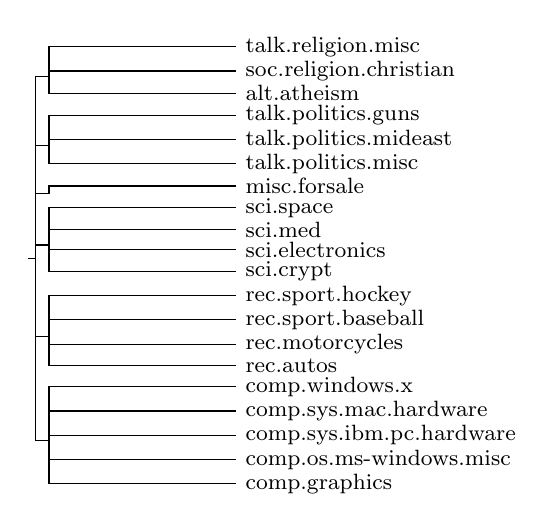
\begin{tikzpicture}
\tikzset{font=\footnotesize}
\tikzset{anchor=base}
\tikzset{sibling distance=-5pt}
\tikzset{level distance=5pt}
\tikzset{frontier/.style={distance from root=75}}
\tikzset{grow=right}
\tikzset{every tree node/.style={anchor=base west}}
\tikzset{edge from parent/.style={draw, edge from parent fork right}}
\Tree [ [ comp.graphics comp.os.ms-windows.misc comp.sys.ibm.pc.hardware comp.sys.mac.hardware comp.windows.x ] [ rec.autos rec.motorcycles rec.sport.baseball rec.sport.hockey ] [ sci.crypt sci.electronics sci.med sci.space ] [ misc.forsale ] [ talk.politics.misc talk.politics.mideast talk.politics.guns ] [ alt.atheism soc.religion.christian talk.religion.misc ] ] 
\end{tikzpicture}
\caption{Topical Clusters}
\label{clusters}
\end{subfigure}%
\begin{subfigure}{.5\textwidth}
\centering
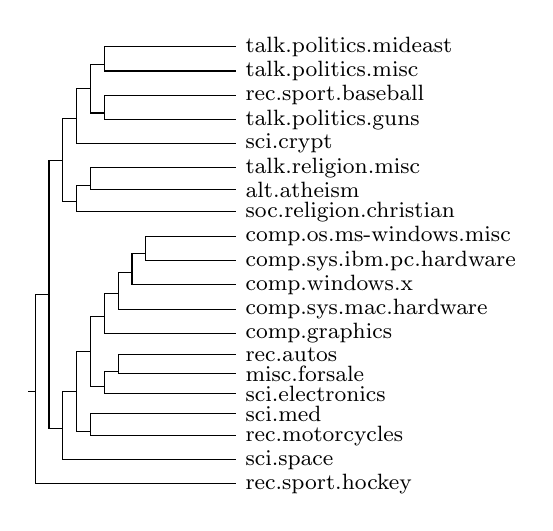
\begin{tikzpicture}
\tikzset{font=\footnotesize}
\tikzset{anchor=base}
\tikzset{sibling distance=-5pt}
\tikzset{level distance=5pt}
\tikzset{frontier/.style={distance from root=75}}
\tikzset{grow=right}
\tikzset{every tree node/.style={anchor=base west}}
\tikzset{edge from parent/.style={draw, edge from parent fork right}}
\Tree [ rec.sport.hockey [ [ sci.space [ [ rec.motorcycles sci.med ] [ [ sci.electronics [ misc.forsale rec.autos ] ] [ comp.graphics [ comp.sys.mac.hardware [ comp.windows.x [ comp.sys.ibm.pc.hardware comp.os.ms-windows.misc ] ] ] ] ] ] ] [ [ soc.religion.christian [ alt.atheism talk.religion.misc ] ] [ sci.crypt [ [ talk.politics.guns rec.sport.baseball ] [ talk.politics.misc talk.politics.mideast ] ] ] ] ] ] 
\end{tikzpicture}
\caption{Learned $\unorderedS$, none}
\label{none-h}
\end{subfigure}
\begin{subfigure}{.5\textwidth}
\centering
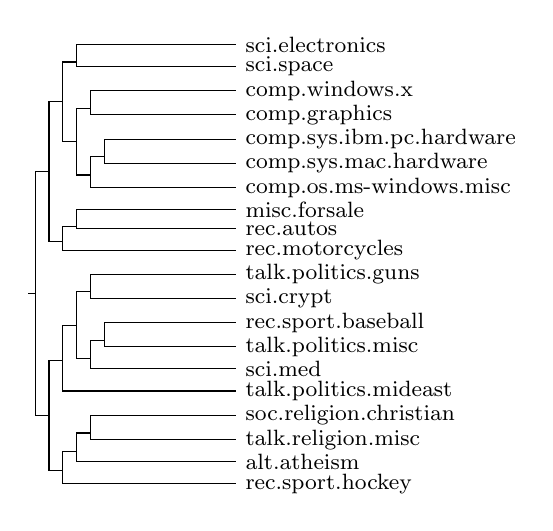
\begin{tikzpicture}
\tikzset{font=\footnotesize}
\tikzset{anchor=base}
\tikzset{sibling distance=-5pt}
\tikzset{level distance=5pt}
\tikzset{frontier/.style={distance from root=75}}
\tikzset{grow=right}
\tikzset{every tree node/.style={anchor=base west}}
\tikzset{edge from parent/.style={draw, edge from parent fork right}}
\Tree [ [ [ rec.sport.hockey [ alt.atheism [ talk.religion.misc soc.religion.christian ] ] ] [ talk.politics.mideast [ [ sci.med [ talk.politics.misc rec.sport.baseball ] ] [ sci.crypt talk.politics.guns ] ] ] ] [ [ rec.motorcycles [ rec.autos misc.forsale ] ] [ [ [ comp.os.ms-windows.misc [ comp.sys.mac.hardware comp.sys.ibm.pc.hardware ] ] [ comp.graphics comp.windows.x ] ] [ sci.space sci.electronics ] ] ] ] 
\end{tikzpicture}
\caption{Learned $\unorderedS$, logical}
\label{logical-h}
\end{subfigure}%
\begin{subfigure}{.5\textwidth}
\centering
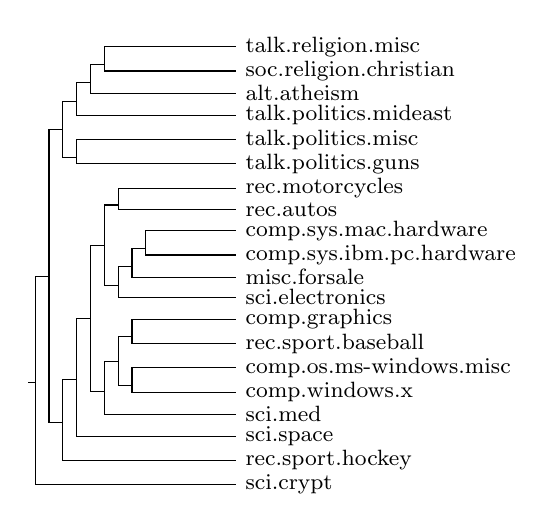
\begin{tikzpicture}
\tikzset{font=\footnotesize}
\tikzset{anchor=base}
\tikzset{sibling distance=-5pt}
\tikzset{level distance=5pt}
\tikzset{frontier/.style={distance from root=75}}
\tikzset{grow=right}
\tikzset{every tree node/.style={anchor=base west}}
\tikzset{edge from parent/.style={draw, edge from parent fork right}}
\Tree [ sci.crypt [ [ rec.sport.hockey [ sci.space [ [ sci.med [ [ comp.windows.x comp.os.ms-windows.misc ] [ rec.sport.baseball comp.graphics ] ] ] [ [ sci.electronics [ misc.forsale [ comp.sys.ibm.pc.hardware comp.sys.mac.hardware ] ] ] [ rec.autos rec.motorcycles ] ] ] ] ] [ [ talk.politics.guns talk.politics.misc ] [ talk.politics.mideast [ alt.atheism [ soc.religion.christian talk.religion.misc ] ] ] ] ] ] 
\end{tikzpicture}
\caption{Learned $\unorderedS$, expected}
\label{expected-h}
\end{subfigure}
\caption{Clusterings of 20 Newsgroup categories.  \ref{clusters} shows
the topical clusters suggested at \url{http://qwone.com/~jason/20Newsgroups/}.
\ref{none-h}, \ref{logical-h}, and \ref{expected-h} show hierarchical
clusterings constructed using distances from the ``ease'' $\mathbf{e}$ 
learned by \ourmethod{} with $\unorderedS$ prediction classes and
``none'' ($\mathbf{1}$), ``logical'', and ``expected'' normalization
constants.}
\label{hierarchies}
\end{figure}

\subsection{Discussion}

Given that \ourmethod{}'s learned cost function approximates the 
relative ease 
of distinguishing between categories in separate topical clusters, 
it is surprising that \ourmethod{} does not give an increased 
accuracy over the SVM baseline in the ``clusters'' column of
 Table~\ref{accuraciesTable}.
This could be an artifact of the 20 newsgroups data set---for example,
the SVM's choice of weights might be near optimal for 
distinguishing between categories in separate topical clusters
given its features, and so there might be nothing that \ourmethod{}
can do to improve these weights. 

Alternatively, it's possible that the \ourmethod{} adjusts its 
weights given the learned costs in a sub-optimal way.  The baseline
multiclass SVM from \citep{crammer2002algorithmic} generalizes the
binary maximum margin-principle from \citep{vapnik1998statistical}
in a way that does not preserve the binary principle's original geometric interpretation.\footnote{There may be an alternative
multi-class SVM formulation which generalizes the
 maximum-margin principle in
way that preserves the original geometric interpretation from the 
binary case.  One way to start thinking about this is to consider
that the difference between feature weights for two classes in the 
multi-class setting form a hyper-plane between those classes, and
the margins around those planes can be maximized.
However, there
are $\binom{|\mathcal{Y}|}{2}$  such hyper-planes, but the current
multi-class SVM only has
$|\mathcal{Y}|$ sets of feature weights (one for each label), and
so the adjustment of one of these planes and its margins has some
effect on the others---not all choices of planes and margins are
possible.  A new 
generalized multi-class maximum margin principle might prescribe
an optimal way to trade-off the margin sizes and errors 
between all of the planes.  This new generalization might even
involve some notion of learned cost, given that we want
to more aggressively maximize the margins between classes which
are more easily distinguishable. It's unclear at this 
point how any of this would work in detail, and we also haven't
reviewed the literature prior to \citep{crammer2002algorithmic}
that attempted other generalizations of the SVM to multi-class 
settings, so they it's possible that they tried something
like this already.
}
Furthermore, \citep{tsochantaridis2004support} shows both  
``slack-rescaling'' and ``margin-rescaling'' methods for incorporating
the cost function into the SVM, and we've only experimented with
the possibly inferior ``margin-rescaling'' method.  Investigations
of the generalization from binary to multi-class, the generalization 
from uniform to
varying cost, and the interaction between these might suggest
ways to use the cost learning to gain feature weights which generalize
better.

A third alternative possible cause for the lack of an accuracy gain by 
\ourmethod{}
is that learned costs do not give an accurate enough encoding of the
 topical clusters, despite the fact that their derived hierarchies seem
 to roughly reflect those clusters.  This failure might be corrected
 through a better choice of normalization constants $\mathbf{n}$.

\section{Related Work}

Here is a list of related work:\footnote{Add details if/when
publishing.}

\begin{enumerate}

\item Self-paced learning \citep{kumar2010self}\footnote{The
objective function used in self-paced learning provided 
some inspiration
for our objective function.}

\item Curriculum learning \citep{bengio2009curriculum}

\item Confidence weighted learning \citep{dredze2008confidence}

\item Inter-annotator agreement cost \citep{plank2014learning}

\item State splitting  \citep{petrov2011coarse}

\item Finite state output encodings \citep{loper2008encoding}

\end{enumerate}

Also, see \url{http://www.cs.cmu.edu/~nasmith/papers/career-proposal-2010.pdf} for more motivations for the cost function
learning.

\subsection{Future Work}

In future work, richer representations of prediction error types
($\mathcal{S}$) might be pursued.  For example, types might be 
constructed based on frequencies of labels, with the rarest labels forming
a group.  For structured output spaces such as natural language
parsing, the domain might suggest
groups of errors; post hoc analysis of $\mathbf{e}$ might, in turn,
suggest ways to improve the model through feature
engineering.\footnote{We note an interesting parallel to the
  \emph{ceteris paribus} reasoning suggested by inspection of
linear model weights $\mathbf{w}$; inspecting $\mathbf{e}$ shows,
``all other things equal,'' a scaling of error types by ease-of-avoidance.}
Our framework is easily extended to let these classes depend on
the input or metadata as well, allowing very rich parameterizations of
learnable cost functions.  Recall that these classes need not be mutually exclusive.

Alternative ways to estimate $\mathbf{n}$ might also be considered,
such as using a more sophisticated model to estimate bounds on error
frequencies in the training set.  More generally, characterizations of
ease might be developed through alternate means, such as the
stability measure from learning theory \citep{mukherjee2006learning},
which might offer insight into the generalizability of predictions
involving a particular label.

We concede that our notion of ``ease'' merges several concepts that
might be treated separately.  These include the reliability of the
labels in training data, the distinctiveness of the labels given the
model family (choice of features), the learnability of each label
given the number of instances it has in the training set, and the
overall similarity of the training distribution to the ``true'' one.
We believe it is an open theoretical question how these various
notions might relate to learning guarantees.

Finally, given our negative results on the text-classification data,
it would be good to experiment with other datasets.  It would be useful
to experiment with synthetic data to try to find out what the model
is doing, or also consider datasets with an even larger number of 
labels where there are even more places for the cost learning to make
a difference.

%\subsubsection*{Acknowledgments}

%Use unnumbered third level headings for the acknowledgments. All
%acknowledgments go at the end of the paper. Do not include 
%acknowledgments in the anonymized submission, only in the 
%final paper. 

\bibliography{refs}

\end{document}
